\chapter[Lezione I]{Lezione I\newline\small{\emph{24/03/2011}}}
	\section{Introduzione informale all'informatica}

Assumiamo, per il momento che l'\emph{algoritmo}\index{algoritmo} sia un processo meccanico che produca dei risultati a partire da dei dati seguendo dei passaggi prestabiliti.
L'\emph{informatica}\index{informatica} è una scienza che permette di risolvere per via algoritmica problemi come i seguenti.


Si\marginpar{Percorso più breve} stabilisca quale percorso deve seguire un aereo per arrivare da un aeroporto ad un altro e, qualora ne esista più di uno, si trovi quello più breve.
Tale problema si può risolvere schematizzando i percorsi e gli aeroporti; operando, cioè, un processo di \emph{astrazione}\index{astrazione} che consiste nell'estrapolare dal problema reale tutti e soli i dati che servano a risolverlo, trascurando dettagli inutili e semplificando così la questione.
Può dunque tornare utile rappresentare gli aeroporti per mezzo di punti e le eventuali rotte che li collegano con dei segmenti.
Fatto ciò, non è più rilevante la struttura geografica dei luoghi o il percorso effettivamente seguito dal mezzo: basta conoscere gli aeroporti, le rotte di collegamento e il loro rispettivo \emph{peso}\index{peso} (ossia la distanza).
Una rappresentazione come quella qui descritta si chiama \emph{grafo}\index{grafo} (vedi il paragrafo~\ref{subsec:grafo} a pagina~\pageref{subsec:grafo}).



Un\marginpar{Problema del ladro} ladro entra in un magazzino ed ha a disposizione solo uno zaino che riesce a sostenere un peso finito con cui trasportare la refurtiva.
Nel magazzino sono presenti oggetti di diverso valore e diverso peso ed il suo scopo è di massimizzare il proprio guadagno cercando di portare via oggetti del maggior valore possibile.
Tale questione si può esprimere in modo più formale considerando uno zaino che possa sopportare un determinato peso $W$ e $N$ oggetti, ciascuno caratterizzato da un peso $w_i$ e un valore $c_i$ con $i\in\Set{1,\dots,N}$.
Si scelga quali di questi oggetti mettere nello zaino per ottenere il maggiore valore senza eccedere nel peso sostenibile dallo zaino stesso \cite{wiki:zaino}.

Una soluzione possibile consiste nello scegliere gli oggetti da portare via in base al loro valore unitario, cioè al rapporto $c_i/w_i$. 
%\[
%V_i=\frac{c_i}{w_i}.
%\]
Un oggetto avrà priorità tanto maggiore quanto più grande sarà il suo valore unitario.


Si\marginpar{Problema dell'ordinamento} hanno \num{50} schedine numerate, indicizzate da numeri \emph{non} progressivi compresi in un range che va da \numrange{1}{e6} e bisogna ridisporle in ordine crescente.
Si ha però a disposizione uno spazio che non permette di vedere i numeri di tutte le schedine contemporaneamente ma solo di appoggiare contemporaneamente due mazzi.

Un procedimento risolutivo potrebbe essere il seguente.
Si estrae una schedina $s_1$ dal mazzo non ordinato e la si appoggia accanto al mazzo stesso, in modo che il suo numero sia visibile.
Successivamente, se n'estrae una seconda $s_2$ e la si confronta con la prima:
\begin{itemize}
	\item
Se $s_1 > s_2$, si pone $s_2$ sopra $s_1$;
	\item
Se $s_1 \le s_2$, si ripone $s_2$ in fondo al mazzo da cui è stata estratta.
\end{itemize}
Si ripete tale procedimento fino a quando il primo mazzo non finisce. In informatica, tale metodo risolutivo prende talvolta il nome di \algo{bubble sort}\index{boubble sort}\index{sort!boubble}.



		\subsection{Efficienza di un algoritmo}
		\label{subsec:eff}
Quando si stende un algoritmo, bisogna cercare di renderlo il più efficiente e performante possibile.
L'efficienza di un algoritmo, come ci si potrebbe aspettare, è inversamente proporzionale al numero di ``calcoli'' che l'esecutore deve compiere per giungere al risultato. 

\begin{table}
	\centering
	\caption[Costo dell'algoritmo \algo{bubble sort}.]{Costo computazionale di un algoritmo \algo{bubble sort} (con $n\in\N\sm\Set{0}$).}
	\label{tab:bubble}
	\begin{tabular}{>$c<$ >$c<$}
		\toprule
\text{Num.~di carte}	&\text{Num.~di confronti}	\\
		\midrule
50			&49				\\
49			&48				\\
48			&47				\\
\vdots 		&\vdots 			\\
n			&n-1				\\
		\bottomrule
	\end{tabular}
\end{table}
La \marginpar{bubble sort} tabella~\ref{tab:bubble} mostra il numero massimo di confronti da compiere (in riferimento alla terza tipologia di problema) tramite un algoritmo di \algo{bubble sort} in relazione al numero di carte che rimangono nel primo mazzo.
In generale, supponendo di avere un mazzo non ordinato di $n$ carte, con $n\in\mathbb{N}$, si hanno $(n-1)+(n-2)+\dots+2+1$ confronti $c$, ossia
\begin{equation}
c_\textup{bs}(n)=\sum_{i=1}^{n-1}i=\frac{(n-2)(n-1)}{2}
\end{equation}
dove, l'ultima uguaglianza è giustificata dall'algoritmo di Gauss per la somma dei primi $n$ numeri naturali.
Pertanto, per $n\to+\infty$, si ha che
\begin{equation}
c_\textup{bs}(n)
%= \sum_{i=1}^{n-1}i=\frac{(n-2)(n-1)}{2}
\overset{n\to\infty}{\thicksim}
\frac{\ n^2}{2}\asymp n^{2},
\end{equation}
ossia raddoppiando il numero di carte il numero di confronti quadruplica.

Esistono \marginpar{merge sort} molti altri metodi d'ordinamento, tra cui l'algoritmo \algo{merge sort}, inventato da John von Neumann nel 1945, che si basa un po' sull'antico detto romano <<divide et impera>> \parencite{wiki:it}.
\begin{figure}
	\centering
%	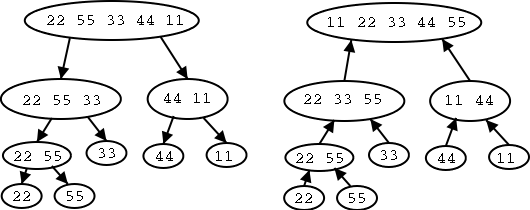
\includegraphics[width=\columnwidth]{immagini/merge_sort}
\subfloat[][Suddivisione.]{
	\begin{tikzpicture}[scale = .85]

\tikzstyle{level 1}=[sibling distance = 25mm]
\tikzstyle{level 2}=[sibling distance = 13mm]
\tikzstyle{level 2}=[sibling distance = 14mm]

\begin{scope}[
	auto=left,
	every node/.style={
		ellipse,
		draw,
		inner sep=2.5pt
	}
]
	\node {$11,22,33,44,55$}
		child {
			node {$22,33,55$}
				child {
					node {$22,55$}
						child { node {$22$} }
						child { node {$55$} }
				}
				child { node {$33$} }
		}
	child {
		node {$11,44$}
			child { node {$44$} }
			child { node {$11$} }
	};
\end{scope}

\draw [thick,->] (2.7,0) -- +(0,-4.5) node [midway,sloped, above] () {divide};

\end{tikzpicture}
}\quad
\subfloat[][Ordinamento.]{
	\begin{tikzpicture}[scale=.85]

\tikzstyle{level 1}=[sibling distance = 25mm]
\tikzstyle{level 2}=[sibling distance = 13mm]
\tikzstyle{level 2}=[sibling distance = 14mm]

\begin{scope}[
	auto=left,
	every node/.style={
		ellipse,
		draw,
		inner sep=2.5pt
	}
]
	\node {$11,22,33,44,55$}
		child {
			node {$22,33,55$}
				child {
					node {$22,55$}
						child { node {$22$} }
						child { node {$55$} }
				}
				child { node {$33$} }
		}
	child {
		node {$11,44$}
			child { node {$44$} }
			child { node {$11$} }
	};
\end{scope}

\draw [thick,<-] (2.7,0) -- +(0,-4.5) node [midway,sloped, above] () {sort};

\end{tikzpicture}
}

	\caption[Merge sort]{Rappresentazione dell'algoritmo \algo{merge sort}.}
	\label{fig:merge}
\end{figure}
Come mostrato in figura~\ref{fig:merge}, si dividono progressivamente i dati di partenza (nel nostro caso, le \num{50} schedine) in due gruppi fino ad ottenerne mazzi da due o un dato.
Se il numero di dati non è divisibile per due, non importa: si avrà almeno un mazzo da una schedina.
Dopo aver suddiviso le schedine, si ordinano progressivamente partendo ``dal basso verso l'alto''.

Per quanto riguarda il costo di tale algoritmo, si devono effettuare all'incirca $\log_2(n)$ suddivisioni e ad ogni passaggio a ritroso bisogna compiere $n$ confronti.
\begin{figure}
	\centering
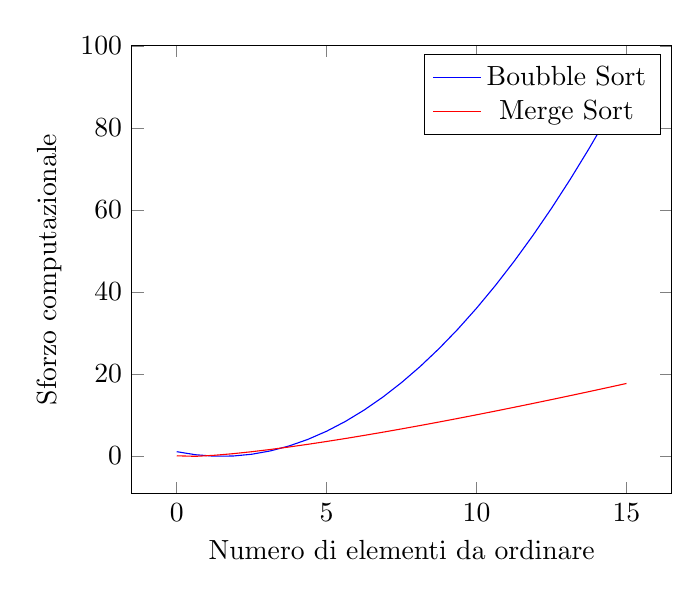
\begin{tikzpicture}
\begin{axis}[
	domain = {0:15},
	xlabel = {Numero di elementi da ordinare},
	ylabel = {Sforzo computazionale}
]
\addplot+[mark=none] {(x-1)*(x-2)/2}; \addlegendentry{Boubble Sort}
\addplot+[mark=none]  {x * log10(x) }; \addlegendentry{Merge Sort}
\end{axis}
\end{tikzpicture}
	\caption{Confronto tra i costi computazionali $c_\textup{bs}$ e $c_\textup{ms}$.}
	\label{fig:costo_cfr}
\end{figure}
Il costo dell'algoritmo è $c_\textup{ms}(n)\simeq n\log_{2}(n)$ e per $n\to+\infty$ si ha
\begin{equation}
c_\textup{bs}(n)\overset{n\to+\infty}{\thicksim} n^{2} \gg n\log_{2}(n) \overset{n\to+\infty}{\thicksim} c_\textup{ms}(n).
\end{equation}
La figura~\ref{fig:costo_cfr} mostra che già per $n \gtrsim \num{10}$ l'algoritmo \algo{merge sort} è più efficiente del \algo{bubble sort}.




	\section{Programma}

Il \emph{programma}\index{programma} è un oggetto che si può presentare sotto varie forme tra cui si distinguono particolarmente le seguenti tre:
\begin{description}
	\item[In corso d'esecuzione] In questo caso, prende il nome di \emph{processo}\index{processo};
	\item[File eseguibile] \`E un file (con estensione \ext{.exe} in \os{Windows}) contenente un insieme d'istruzioni comprensibili dall'unità di calcolo.
\`E scritto in un linguaggio che prende il nome di \lang{Assembly} o \lang{Linguaggio Macchina} e, come si intuisce, non è fatto per essere letto ed interpretato dall'uomo.
Quando un file eseguibile viene lanciato si traduce in un processo;
	\item[Codice sorgente] \`E un file di testo contenente istruzioni comprensibili anche all'uomo ed è scritto in un \emph{linguaggio di programmazione}.
Per ottenere un file eseguibile dal codice sorgente c'è bisogno di ``tradurlo'' tramite un processo che, per ragioni storiche, prende il nome di \emph{compilazione}\index{compilazione}.\footnote{Per maggiori dettagli, si rimanda a degli appunti sul sito del prof.~Bernardinello all'indirizzo \url{http://www.mc3.disco.unimib.it/lif/Dep/vigcc.pdf}}
\end{description}